\documentclass[11pt]{article}
\usepackage{mypackages}
\begin{document}

\maketitle

\section{Deep Learning}


\subsection{Intro}

Deep Learning is a topic in Machine Learning (ML). In deep learning we using An Artificial Neural Network (ANN), which is a computation model inspired by the human brain. The idea in an Artificial Neural Network is that we building a network of \textit{neurons} which is connected to each other, and the learning is done by adjusting the connection between these neurons, the connection parameter between two neurons is called \textit{weights} and by adjusting these weights we can optimize the network for solving a problem.


\subsubsection{Layers, neurons}

The idea in an Artificial Neural Network is that we building a network of \textit{neurons}. A neuron is the basic unit used for computation in a neural network, the neuron receives some input either from the environment or from other neurons and compute an output. Each input neuron have a value and a \textit{weight}, which is assigned to the relative importance to the other input neurons. The neuron applies a function $f$ to the weighted sum of the input neurons. So the output of a neuron is $f(w_{1} \cdot X_{1} + w_{2} \cdot X_{2} + \cdots + w_{n} \cdot X_{n})$, and can be illustrated as
\begin{figure}[!h]
    \centering
    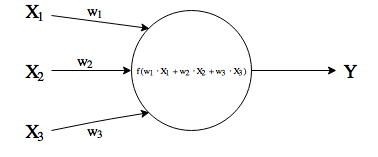
\includegraphics[scale = 0.5]{include/neuron.png}
    \caption{Illustration of neuron}
    \label{fig:neuron}
\end{figure}
\\
The function $f$ applied on the weighted sum of the input, is called an \textit{activation function}. An activation function takes the weighted sum and perform a mathematical operation on it. We are using these activation functions in this project:
\\ \\
\textbf{ReLU:} ReLU stands for Rectified Linear Unit. ReLU return the maximum of $0$ and $x$:
\begin{equation}
f(x)=\max(0,x)
\end{equation}
And is illustrated as
(INDSÆT BILLEDE)




\end{document}
